 \documentclass{article}
\usepackage[letterpaper, top=0.2in, left=0.45in, right=0.45in, bottom=0.2in]{geometry}
\usepackage{amsmath, amssymb}
\usepackage{tcolorbox}
\usepackage[dvipsnames]{xcolor}
\usepackage{ifthen}
\tcbuselibrary{listings,breakable}
\usepackage{float} % Allows precise placement of floating objects
\usepackage{tikz} % Core TikZ package
\usepackage{pgfplots} % For statistical plots
\pgfplotsset{compat=1.18} % Ensure compatibility

\usepackage{comment}

\usetikzlibrary{positioning, shapes, calc, backgrounds, decorations.pathreplacing, arrows.meta, plotmarks}

% Define a new command for a centered floating blank text box
\newcommand{\blankbox}[2][3cm]{%
    \vspace{-0.5em}
    \begin{figure}[H]
        \makebox[\linewidth]{% Ensures the box extends to full line width
            \begin{tcolorbox}[
                colback=white, 
                colframe=black, 
                width=#2, % Adjusting for A4 paper margins
                height=#1,
                boxrule=0.2mm
            ]
            \end{tcolorbox}
        }
    \end{figure}
    \vspace{-2em}
}

% Define a new boolean for showing or hiding answers
\newboolean{showanswers}
\setboolean{showanswers}{false}  % Set to true to show answers, false to hide answers

% Define the command to conditionally display answers
\newcommand{\answer}[1]{
    \ifthenelse{\boolean{showanswers}}{
        \begingroup
        \color{MidnightBlue}
        \begin{tcolorbox}[colback=white, colframe=MidnightBlue, title=Solution, fonttitle=\bfseries, breakable, fontupper=\color{MidnightBlue}]
        #1
        \end{tcolorbox}
        \endgroup
    }{}
}
%%%%%%%%%%%%%%%%%%%%%%%%%%%%%%%%%%%%%%%%%%%%%%%%%%%%%%%%%%%%%%%%%%%%%%%%%%%%%%%%%%%%%%%%%%%%%%%

\begin{document}
%\setlength{\parindent}{0pt} % remove indentation in the whole document
\pagenumbering{gobble} % Suppress page numbers
 \hspace{1em} \vspace{-1.7em}
\begin{center}
   \Large   POL201.01 - Midterm Spring 2025
\end{center}

\vspace{1em}
\noindent\textbf{First and Last Name:} \underline{\hspace{8cm}}  \quad  \textbf{Student ID:} \underline{\hspace{4.4cm}} 

\vspace{0.7em}
\noindent\textbf{Instructions:} 

\vspace{-0.8em}
\begin{itemize}
    \setlength{\itemsep}{-0.35em}
    \item Turn off and put away your phone and any electronic devices.
    \item You have from \textbf{9:35 AM to 10:45 AM} to complete the midterm.
    \item Show all your work. Partial credit may be awarded.
    \item Read each question carefully and manage your time wisely.
    \item Write your answers in the space provided. If you need additional space for scratch work, you may use the back of the pages, but only answers written in the designated areas will be graded.
    \item If you have any questions, raise your hand and ask the instructor.
\end{itemize}
\vspace{-1.1em}
\noindent\rule{\linewidth}{0.4pt} % Horizontal line to separate this section from the exam content

\section*{Section 1 (11 points total)}

\noindent\textbf{Instructions:}  
Suppose an artificial intelligence (AI), like ChatGPT, is playing \emph{four consecutive rounds} of the card game \emph{Uno} against a \emph{sophisticated, but rule-based} computer algorithm. Unlike the AI, which adapts its strategy dynamically, the rule-based algorithm follows a fixed decision-making process (i.e., the algorithm is just a set of step-by-step instructions telling the computer exactly how to respond to each card or game event).

We run \emph{one billion} simulations of these four-round matches. Based on these simulations, we estimate the \textbf{probability mass function (PMF)} of $X$, the number of rounds won by the AI in a given match:
\[
P(X = k) = p_k, \quad k = 0,1,2,3,4
\]
where:
\[
\begin{array}{c|c|c|c|c|c}
X & 0 & 1 & 2 & 3 & 4 \\\hline
P(X = k) & 0.10 & 0.25 & 0.30 & 0.20 & 0.15 \\
\end{array}
\]

\begin{enumerate}
    \item \underline{Question 1.1}: Compute the \emph{expected number of rounds won} by the AI in a match. Then, \emph{explain what this value represents in the context of the game}. How does this help us understand the AI's performance?  (\textbf{6 points})
        \blankbox[6cm]{1.06\textwidth}  
    \item \underline{Question 1.2}: Compute the \emph{probability that $X$ is higher than $E[X]$}. \emph{Interpret} this probability in the context of the AI's performance in individual matches. (\textbf{5 points})
        \blankbox[5cm]{1.06\textwidth}

        
\end{enumerate}

    %\item \underline{Question 3.3}: \emph{Interpretation}: If you were designing a new AI to play Uno, would you say that the current AI is dominant over the rule-based algorithm? Justify your answer using the probabilities given. \blankbox[5cm]{1.06\textwidth}  
%%%%%%%%%%%%%%%%%%%%%%%%%%%%%%%%%%%%%%%%%%%%%%%%%%%%%%%%%%%%%%%%%%%%%%%%%%%%%%%%%%%%
\newpage
\section*{Section 2 (5 points per question)}

\noindent\textbf{Instructions:}  
The dataset below shows the number of hours a random sample of 19 college students spent consuming political news over the past week.
\[
\{\,0,0,0,\;\,1,1,1,\;\,2,2,2,2,\;\,3,3,3,\;\,4,4,\;\,5,\;\,6,6,\;\,11\}.
\]
\noindent 
For this dataset, the following aggregates or summaries are provided:
\[
\sum x_i = 56, \quad \sum (x_i - \bar{x})^2 = 130.95, \quad n = 19,  \quad  Q_1 = 1,\, Q_2 = 2, \, Q_3 = 4 \quad \text{($Q_k$ is the $k$-th Quartile)}
\]

\begin{comment}
{
    "sum_x": 56,
    "sum_x_squared": 296,
    "sum_x_minus_mean_squared": 130.95,  # Rounded from 130.9473684210526
    "n": 19,
    "Q1": 1.0,
    "Q2": 2.0,
    "Q3": 4.0
}
\end{comment}

\begin{comment}
\begin{center} 
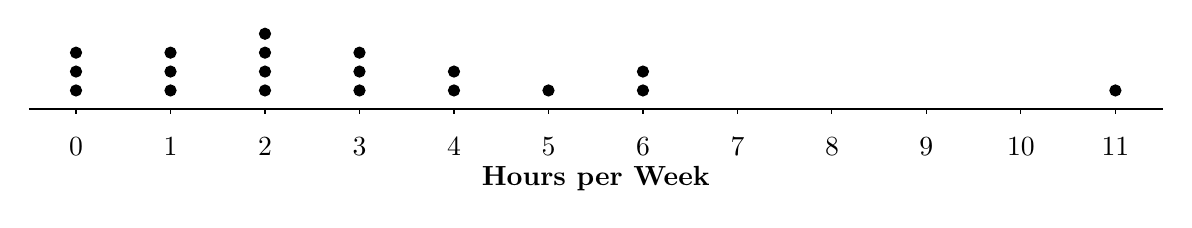
\begin{tikzpicture}[x=1.2cm, y=1.2cm]

    % Draw horizontal axis
    \draw[thick] (-0.5,0) -- (11.5,0);

    % Tick marks and x-axis labels
    \foreach \x in {0,1,2,3,4,5,6,7,8,9,10,11} {
        \draw (\x, 0) -- (\x, -0.05);
        \node[below] at (\x, -0.2) {\x};
    }
    \node[below] at (5.5, -0.5) {\textbf{Hours per Week}};

    % Plot the 19 data points

    % 0's (3 occurrences)
    \draw[fill] (0, 0.2) circle (2pt);
    \draw[fill] (0, 0.4) circle (2pt);
    \draw[fill] (0, 0.6) circle (2pt);

    % 1's (3 occurrences)
    \draw[fill] (1, 0.2) circle (2pt);
    \draw[fill] (1, 0.4) circle (2pt);
    \draw[fill] (1, 0.6) circle (2pt);

    % 2's (4 occurrences)
    \draw[fill] (2, 0.2) circle (2pt);
    \draw[fill] (2, 0.4) circle (2pt);
    \draw[fill] (2, 0.6) circle (2pt);
    \draw[fill] (2, 0.8) circle (2pt);

    % 3's (3 occurrences)
    \draw[fill] (3, 0.2) circle (2pt);
    \draw[fill] (3, 0.4) circle (2pt);
    \draw[fill] (3, 0.6) circle (2pt);

    % 4's (2 occurrences)
    \draw[fill] (4, 0.2) circle (2pt);
    \draw[fill] (4, 0.4) circle (2pt);

    % 5's (1 occurrence)
    \draw[fill] (5, 0.2) circle (2pt);

    % 6's (2 occurrences)
    \draw[fill] (6, 0.2) circle (2pt);
    \draw[fill] (6, 0.4) circle (2pt);

    % 11's (1 occurrence)
    \draw[fill] (11, 0.2) circle (2pt);

\end{tikzpicture}
\end{center}
\end{comment}

\begin{enumerate}
    \item \underline{Question 2.1}: Calculate the \emph{average} number of hours spent on political news.  \emph{Interpret this number}.
        \blankbox[3.5cm]{1.06\textwidth}  
    \item \underline{Question 2.2}: Identify the \emph{median}. \emph{Justify your answer}.
        \blankbox[5cm]{1.06\textwidth}
    \item \underline{Question 2.3}: Determine the \emph{mode}. \emph{Justify your answer}.
        \blankbox[5cm]{1.06\textwidth}
    \item  \underline{Question 2.4}: Which measure, the \emph{mean} or the \emph{median}, better represents the central value of this dataset?  \emph{Justify your answer}.
        \blankbox[5cm]{1.06\textwidth}
\end{enumerate}

\begin{comment}
\item  \underline{Question 2.5}: According to the sample data, what is the probability that a student’s political-news consumption is greater than or equal to 0.90 standard deviations above the sample mean? \emph{Justify your answer}. (\emph{Hint: Use the Z-score transformation equation to find the implicit value for $x$ when $Z=0.90$, given $\bar{x}$ and $s$)}
\blankbox[4cm]{1.06\textwidth}
\end{comment}

%%%%%%%%%%%%%%%%%%%%%%%%%%%%%%%%%%%%%%%%%%%%%%%%%%%%%%%%%%%%%%%%%%%%%%%%%%%%%%%%%%%%
\newpage
\section*{Section 3 (3 points per question)}

\noindent\textbf{Instructions:}  
For each \emph{statement} below, determine whether it is \texttt{True} or \texttt{False} and circle your choice. Then, provide a clear and well-reasoned explanation to support your answer. Justification is valued more than simply selecting the correct option, with 1 point awarded for the correct selection and 2 points for a well-explained justification. \emph{Clearly explain the formulas you use and the calculations you perform}.


\begin{enumerate}

%%%%%%%%%%%%%%%%%%%%%%%%%%%%%%%
\item \underline{Question 3.1}: A survey was conducted to understand the voting preferences of urban and rural residents in a state ahead of the upcoming gubernatorial election. It included 1,000 randomly selected participants, with 700 from urban areas and 300 from rural areas. Among urban residents, 350 supported the current governor, while 180 rural residents also expressed their support.

\noindent
\begin{tabular}{p{0.75\textwidth} p{0.04\textwidth} p{0.15\textwidth}}
\textbf{Statement}: \emph{``Given this data, an urban resident is more likely to support the current governor compared to a rural resident."} 
& \centering  & \centering \texttt{True} \quad  \texttt{False} \\
\end{tabular}
\vspace{-0.9em}
    \blankbox[5cm]{1.06\textwidth} % A box with 4cm height and full text width
    \answer{
    placeholder
    }

%%%%%%%%%%%%%%%%%%%%%%%%%%%%%%%
\item \underline{Question 3.2}: A survey was conducted to examine the relationship between voting behavior and support for a new healthcare policy among adults in a city. Based on the survey data, the following probabilities were reported: \emph{i}) The probability that an adult supports the new healthcare policy is 40\%; \emph{ii}) The probability that an adult voted in the last election is 60\%; \emph{iii}) The probability that an adult supports the policy given that they voted is 50\%.  

\noindent
\begin{tabular}{p{0.75\textwidth} p{0.04\textwidth} p{0.15\textwidth}}
\textbf{Statement}: \emph{``The probability that an adult both supports the new healthcare policy and voted in the last election is higher than 1/4."} 
& \centering  & \centering \texttt{True} \quad  \texttt{False} \\
\end{tabular}
\vspace{-0.9em}
    \blankbox[5cm]{1.06\textwidth} % A box with 4cm height and full text width
    \answer{
    placeholder
    }

%%%%%%%%%%%%%%%%%%%%%%%%%%%%%%%
\item \underline{Question 3.3}:  A jury of three members is deciding on a verdict. Each juror makes a statistically independent decision. Let \( X_i \) be a binary random variable representing the decision of juror \( i \), where \( X_i = 1 \) if the juror votes guilty and \( X_i = 0 \) if the juror votes not guilty.   The probability that each juror votes guilty is as follows: \( P(X_1 = 1) = 0.3 \), \( P(X_2 = 1) = 0.4 \), and \( P(X_3 = 1) = 0.2 \).  

\noindent
\begin{tabular}{p{0.75\textwidth} p{0.04\textwidth} p{0.15\textwidth}}
\textbf{Statement}: \emph{``The probability that at least one juror votes guilty is greater than 80\%."} 
& \centering  & \centering \texttt{True} \quad  \texttt{False} \\
\end{tabular}
\vspace{-1.4em}
    \blankbox[5cm]{1.06\textwidth}  
    \answer{  
        placeholder  
    }  
    

\end{enumerate}

\end{document}


